%!TEX root = ../NCVC2.tex

\mysection{オフセット交点除去}

\vspace*{1.5zh}
 手動で内外の輪郭を変更しても,輪郭同士の交点はリアルタイムには計算されません.
複雑な計算になるので応答性を高めるための措置です.
当然ながらこのまま加工データを作ると不具合があるので,手動で調整作業をした場合だけ,
\menu{編集>加工指示>オフセット交点除去} の処理を行ってください.
図\ref{fig:offset1.png} の確認ダイアログでOKボタンを押すと,

\begin{figure}[H]
\centering
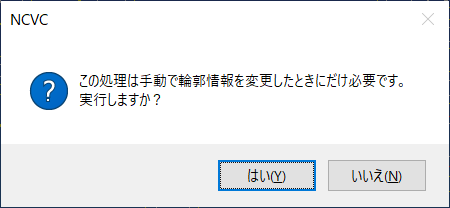
\includegraphics{No4/fig/dialog.png}
\caption{オフセット交点除去の確認ダイアログ}
\label{fig:offset1.png}
\end{figure}

図\ref{fig:offset2.png} のように,めでたく輪郭が計算されました.

\begin{figure}[H]
\centering
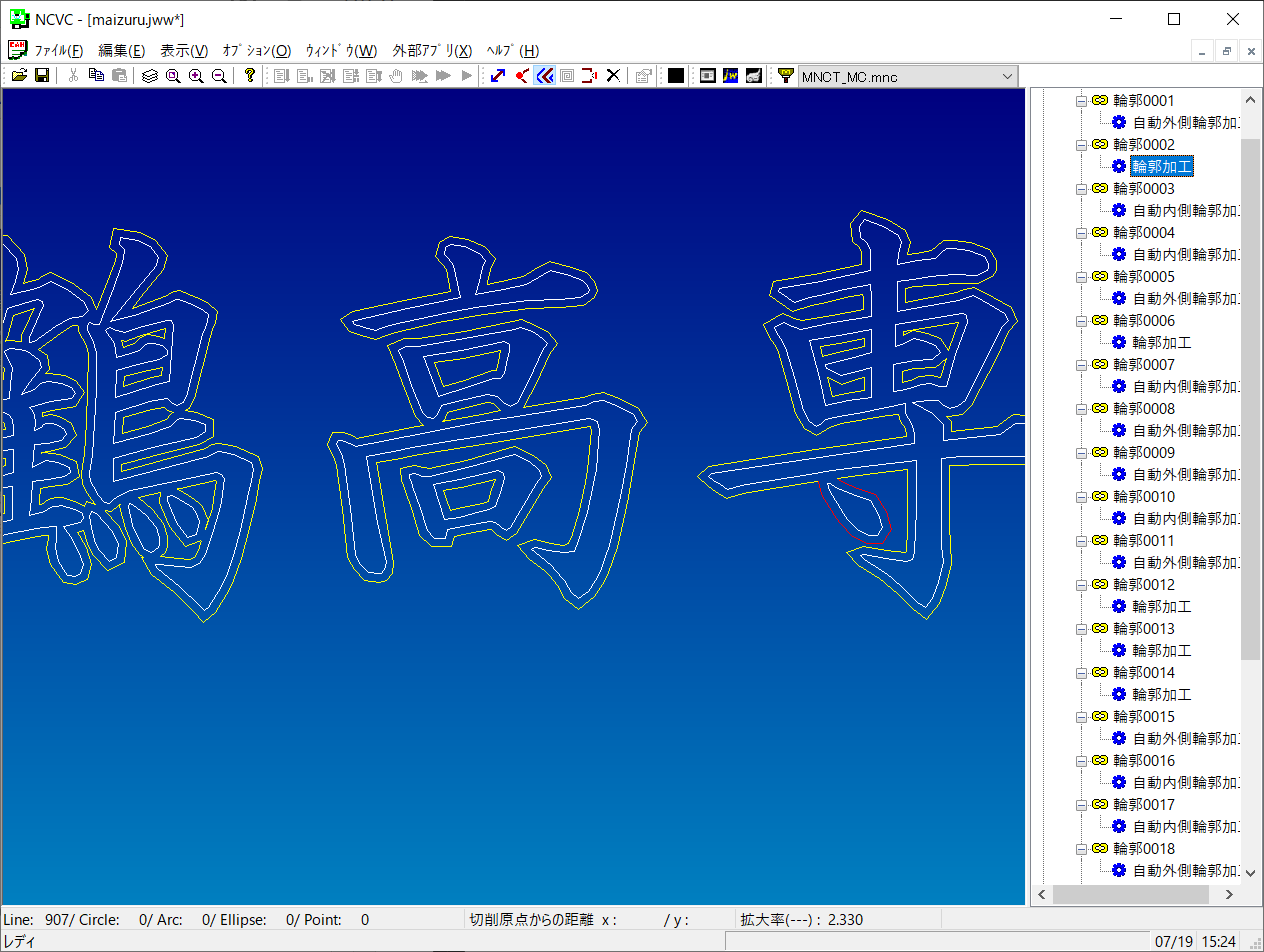
\includegraphics[scale=0.5]{No4/fig/offset.png}
\caption{オフセット交点除去の結果}
\label{fig:offset2.png}
\end{figure}

 この状態で\menu{ファイル>加工情報の保存(Ctrl+S)} しておくと,
輪郭オフセットなどの加工指示がNCVC独自形式の CAM ファイルとして保存できます.